\chapter{Methodology}

\begin{justify}
Methods for developing software are systematic approaches to completing a software project. Approaches that are both effective and practical often combine a set of clearly defined stages with a conceptual approach to design or process. There are many different methods to go about developing software. As much as one might wish otherwise, there is a profound lesson to be learned from all available approaches. Before settling on a certain approach, it's wise to be familiarized with the most popular software development approaches. The most well-known software development approaches are the Waterfall Approach, the Iterative Approach, and the Incremental Approach. In the following, I briefly discuss each method before presenting the methodology used for this project.

\vspace{0.25cm}
\newendline The traditional waterfall method is a method that follows a linear and sequential progression and divides the software development process into a number of discrete stages in a chronological manner. Planning, analysis, design, implementation, testing, deployment, and maintenance are the steps that make up the traditional waterfall approach. The most significant benefit of using this method is that it makes it possible to have a well-defined and well-organized process of development, where each phase builds upon the one that came before it. However, a potential downside is that once a phase is over, there is little room for iteration or change.

\begin{figure}[H]
    \centerline{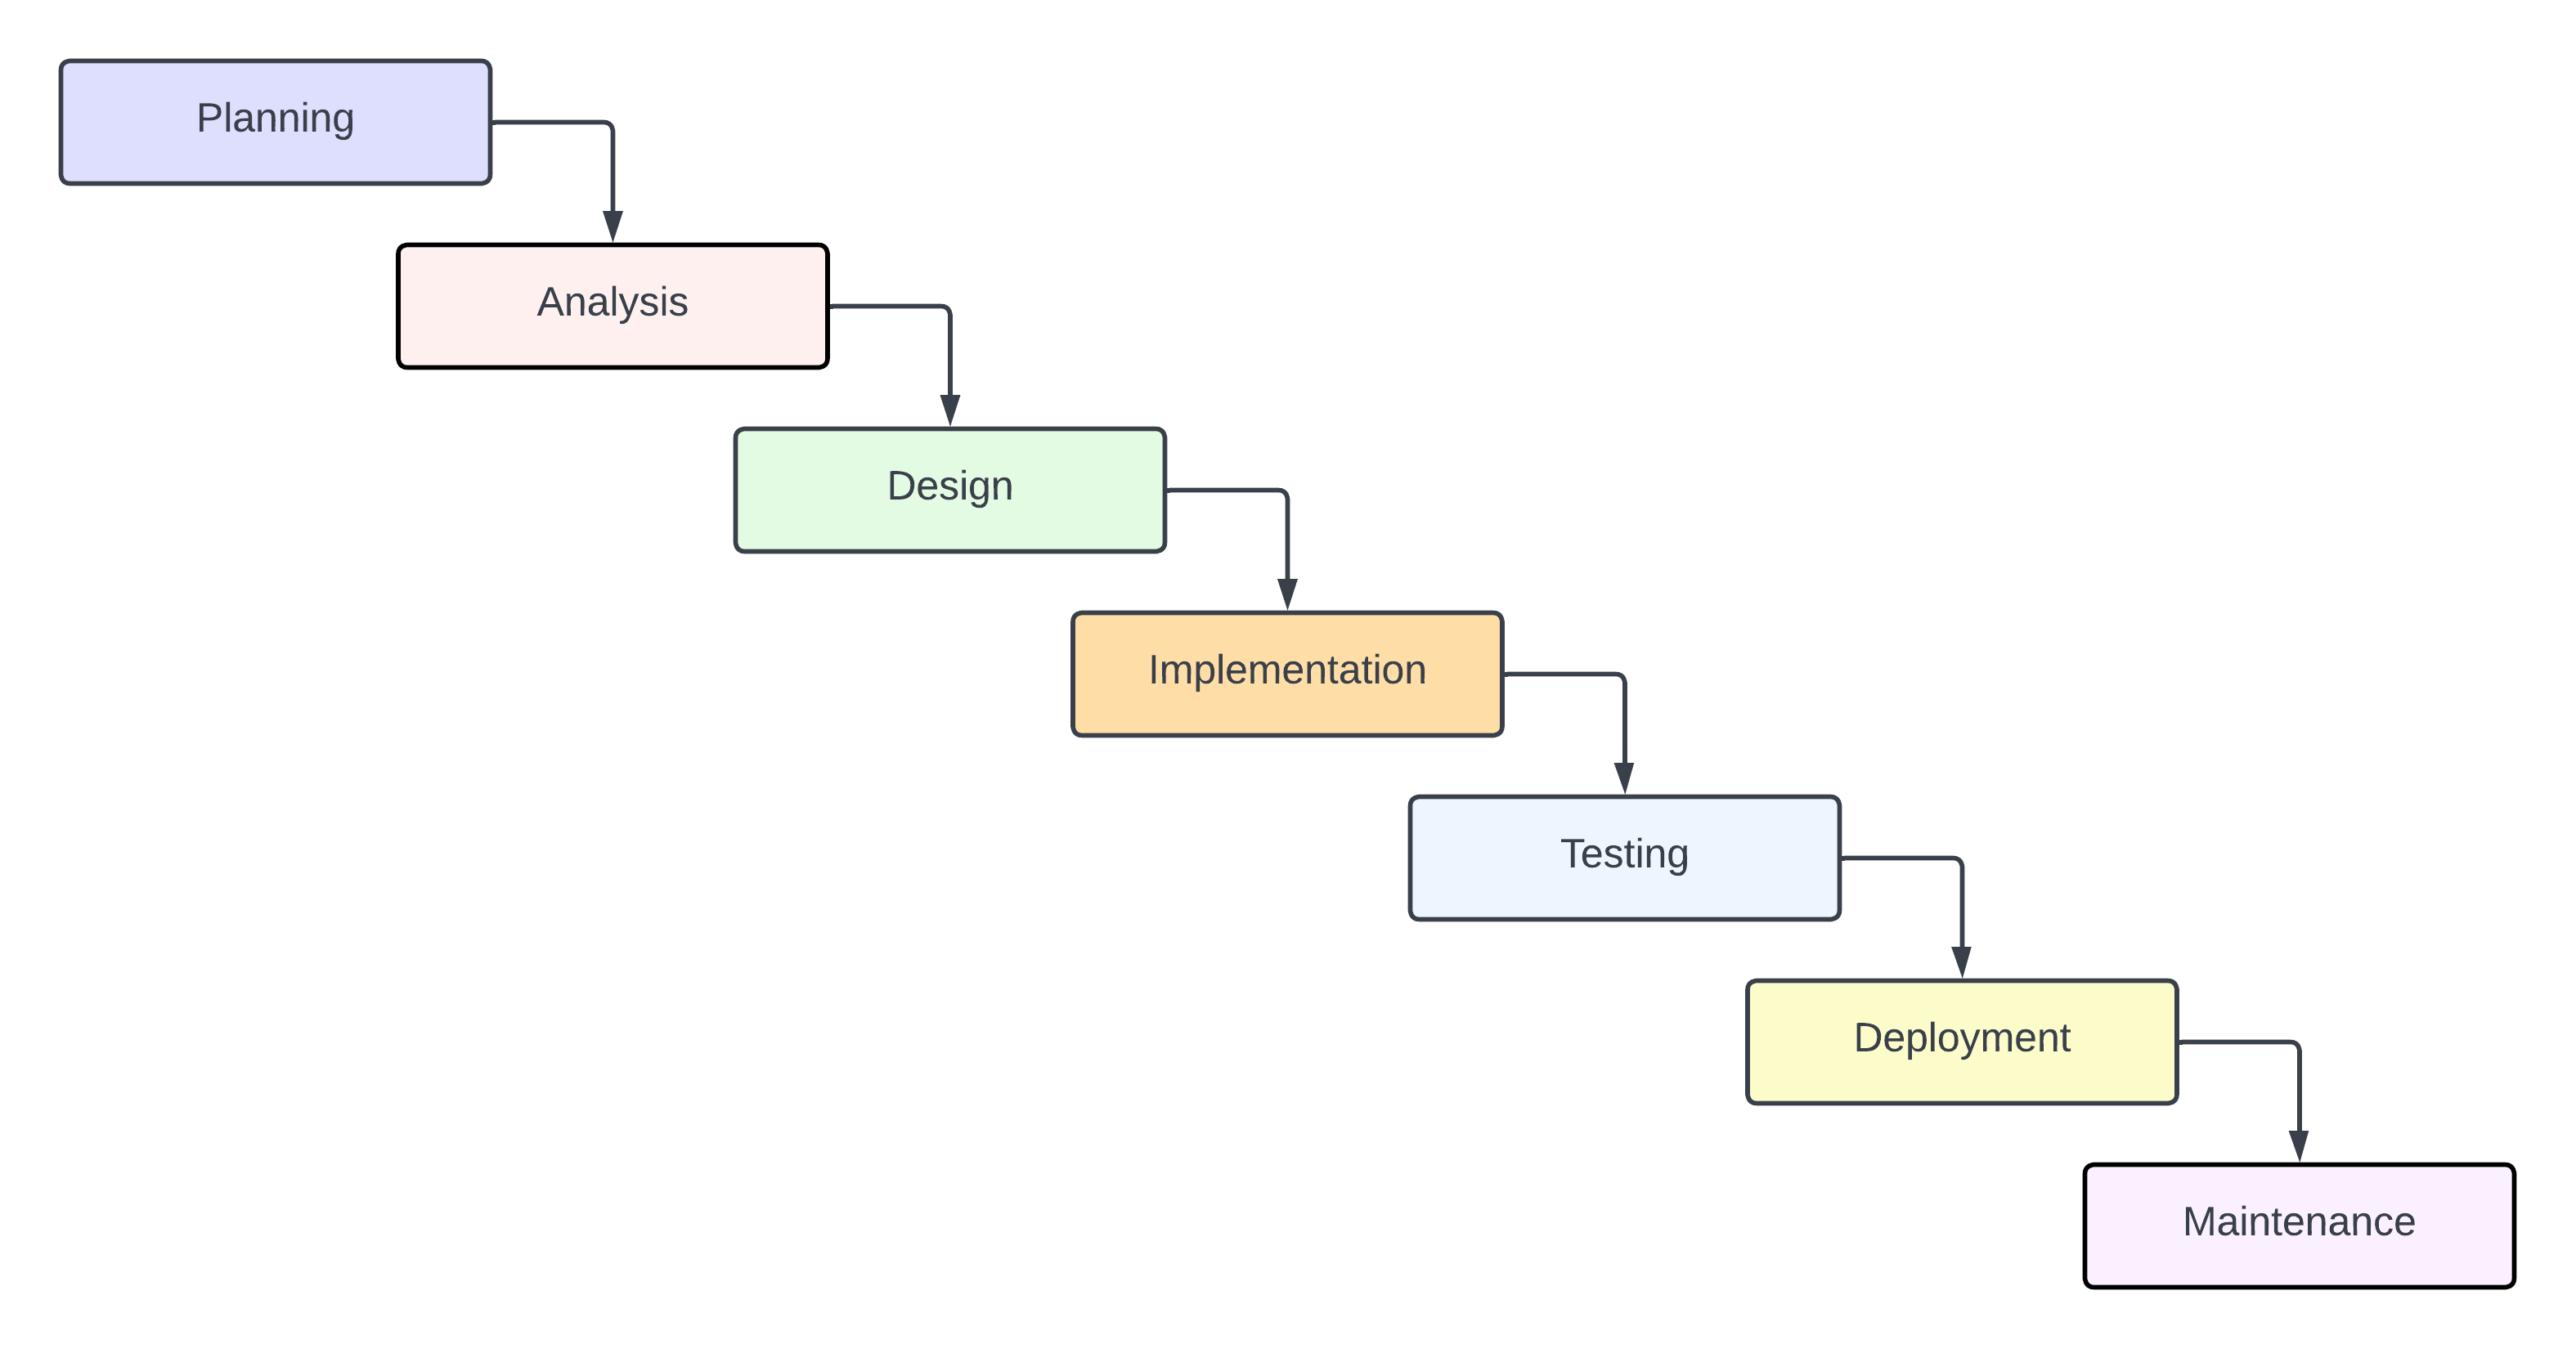
\includegraphics[width=140mm,scale=1]{figures/methodology/Waterfall.png}}
    \caption{Waterfall approach}
    \label{Waterfall}
\end{figure}

\noindent
Approaches to the development of software that are iterative entail the repetition of cycles, sometimes known as iterations, of planning, implementing, and evaluating. As a result, this enables a larger degree of flexibility, as well as the chance to make modifications and enhancements while the product is still being developed. However, due to the fact that the scope of the project may undergo major changes throughout the course of its duration, it may be more challenging to manage and control.

\vspace{0.25cm}
\newendline The method of developing software incrementally entails slicing the whole process of development into smaller pieces, which are referred to as increments, and providing a version of the system that is operational at the completion of each iteration. Because of this, a strategy that is more flexible and iterative is possible, since each increment may be tweaked and improved upon depending on the comments and suggestions of users. Nevertheless, it may be more difficult to manage and organize, particularly if the project involves a large number of increments.

\begin{figure}[H]
    \centerline{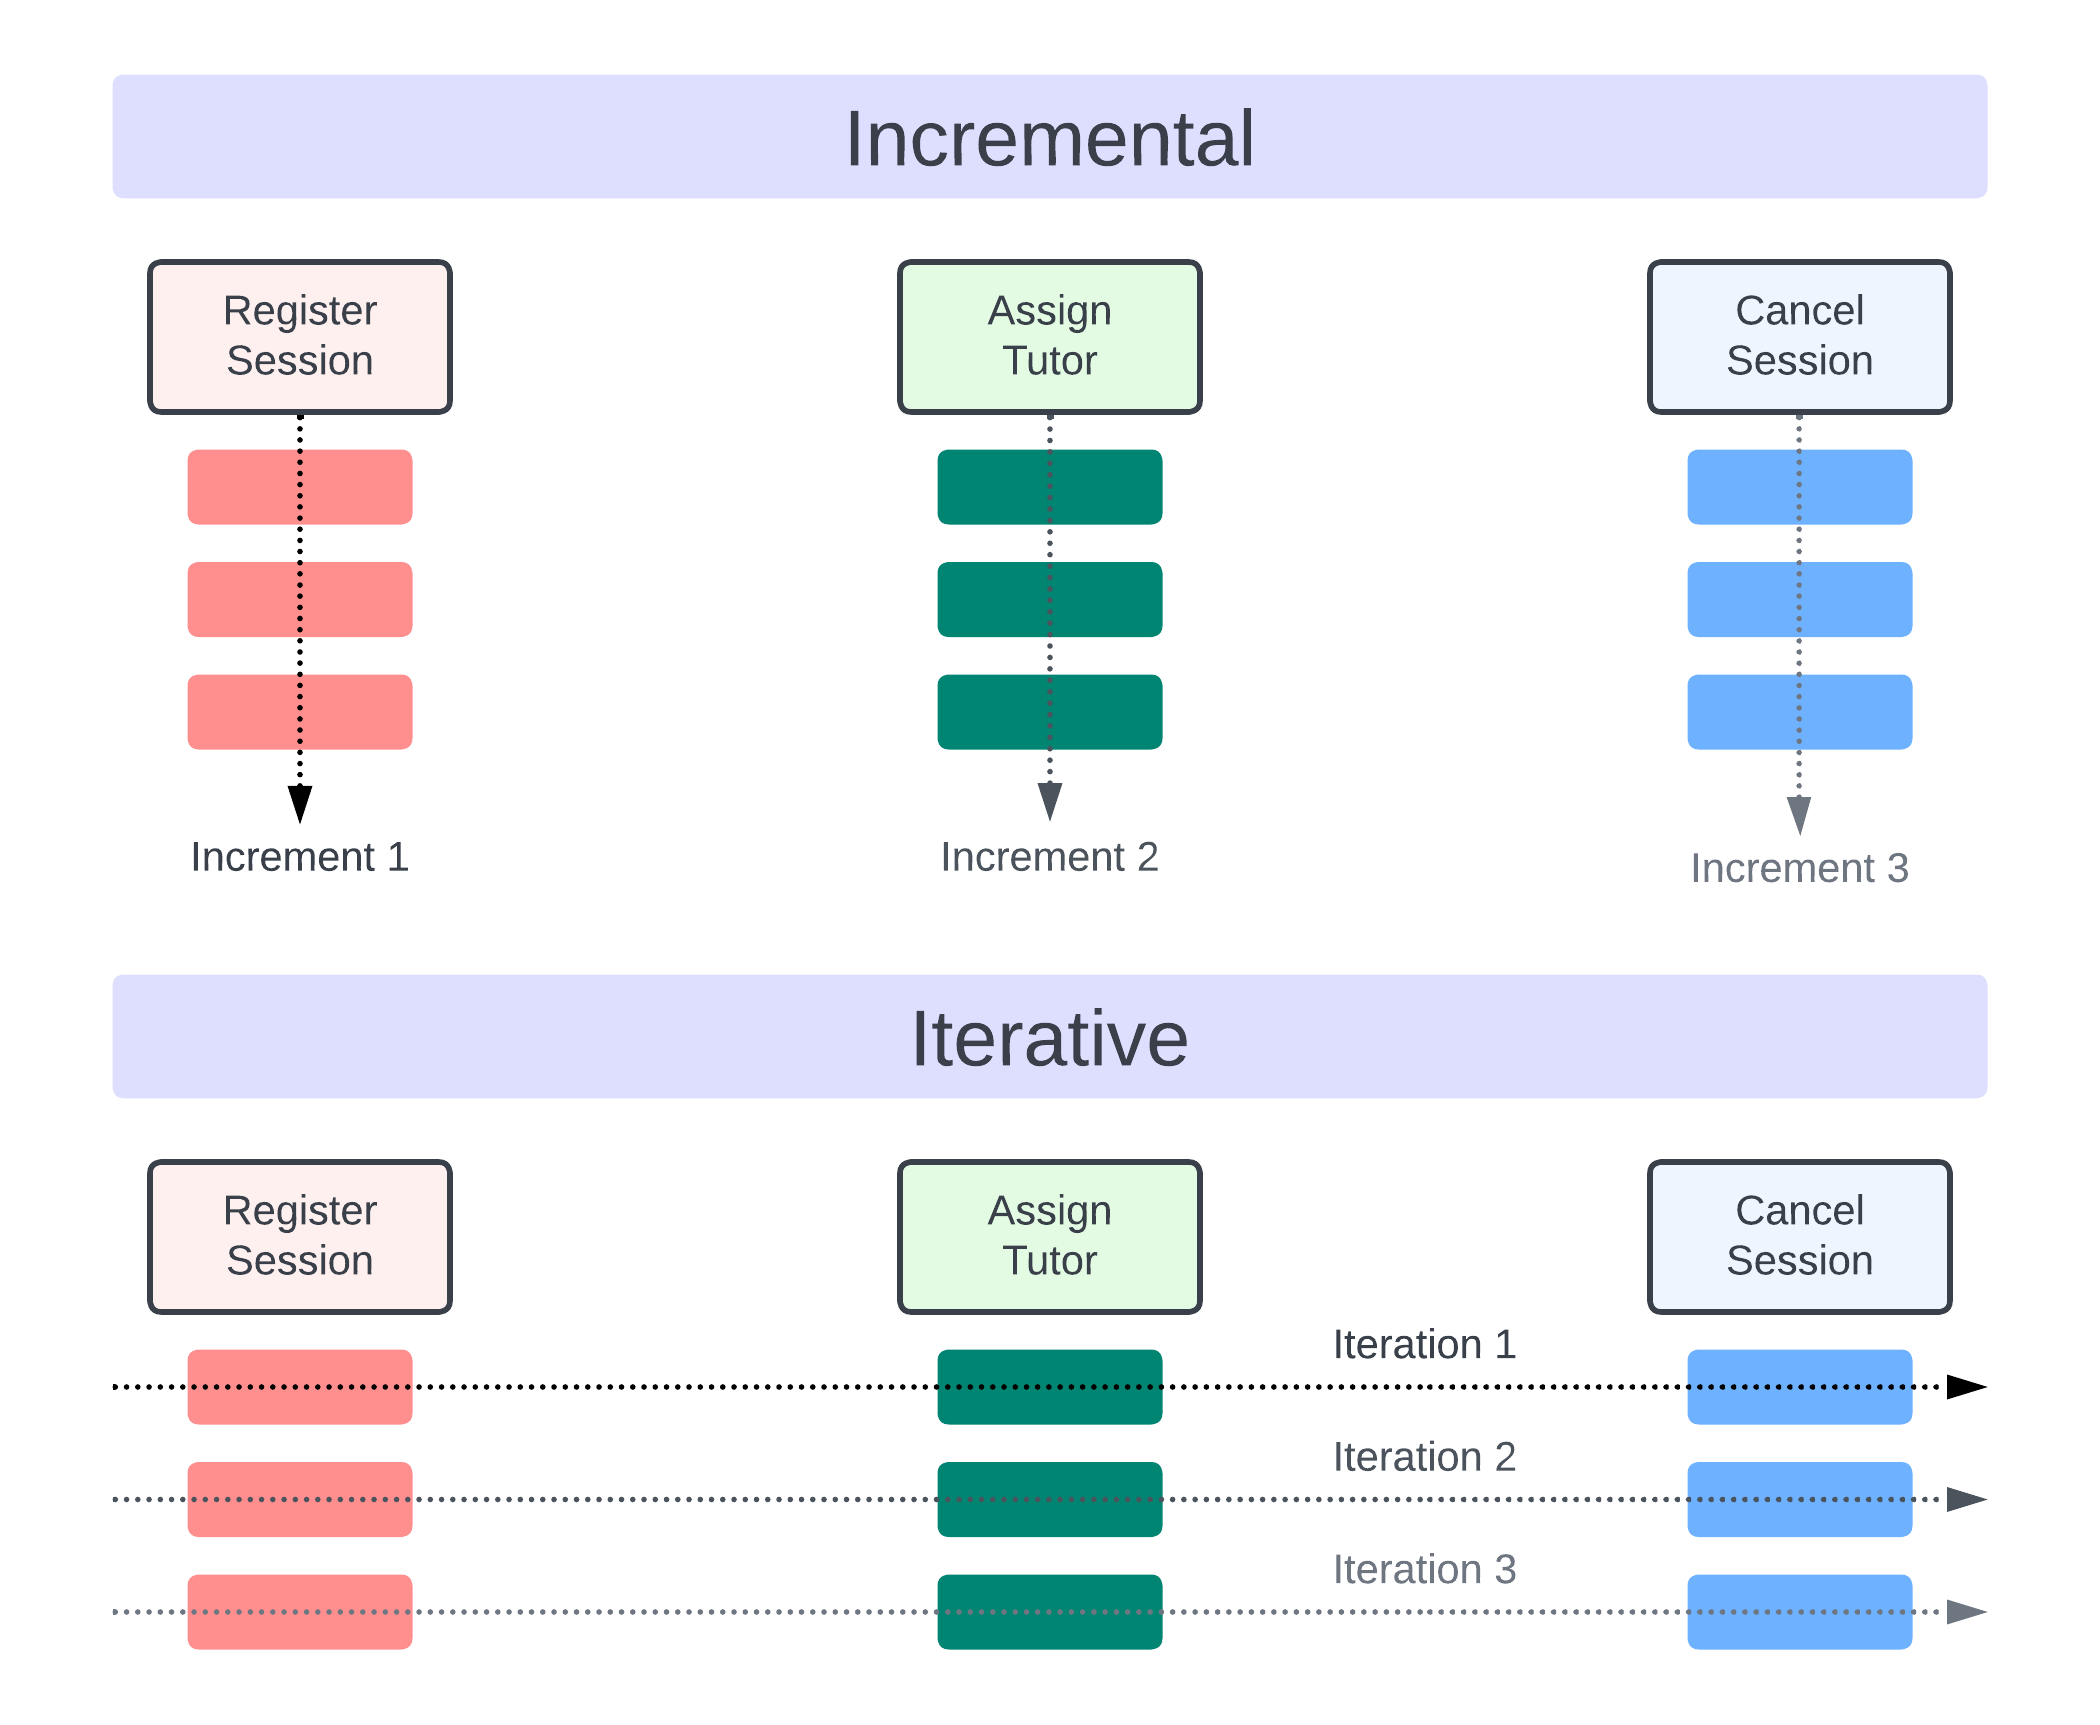
\includegraphics[width=150mm,scale=1]{figures/methodology/IncrementalVsIterative.png}}
    \caption{Difference between incremental and iterative}
    \label{IncrementalVsIterative}
\end{figure}

\noindent
The methodology for developing this application is based on a customized version of the waterfall model. I follow the standard stages of the waterfall model for this project; however, I have made certain adjustments so that they are more closely aligned with the particular needs and requirements of this project. The adjustments are including the followings:
\vspace{0.25cm}
\begin{enumerate}
    \item Deployment and maintenance stages of the traditional waterfall are omitted based on consultation with my supervisor.
    \item Testing stage does not start after implementation rather it will start as soon as the requirements are gathered and continues throughout the project.
\end{enumerate}

\vspace{0.25cm}
\newendline Planning, analysis, design, implementation, and testing are the different stages that are included in this customized waterfall model. Therefore, it is important to highlight what each stage includes, below here, each stage is explained.
\vspace{0.25cm}
\newendline As the initial stage in the process of developing the project, feasibility studies are being carried out. The purpose of these studies is to investigate the practicability of the project that is going to be carried out in terms of its technical, economic, and cultural feasibility. The following stage is the planning phase, which comes at the beginning of the software development life cycle (SDLC) and is hence the first phase. In this phase, I define a thorough project plan that describes the tasks, resources, and timetable for the development process. In addition, I define the stakeholders and risks analysis of the project.
\vspace{0.25cm}
\newendline Following the planning phase, I conduct the analysis phase. During this phase, I collect the requirements for the application, which include the needs and expectations of the stakeholders, and document those requirements by creating use cases and activity diagrams. The application's functionality, performance, and overall quality are all determined by the requirements; thus, I treat them as the application's premise. In order to guarantee that the application will satisfy the criteria of the stakeholders, I stay in contact with the stakeholders to validate all of the requirements at the end of this stage.
\vspace{0.25cm}
\newendline As mentioned above, instead of delaying the start of testing until the later phases of the development process, I start the testing stage during the analysis phase. This enables me to validate the completeness and correctness of the requirements as soon as they are gathered, and it also enables me to identify and rectify any concerns early on in the process. The functional requirements of the application are the primary focus of the testing activities that take place during the analysis phase. These activities include testing methods such as requirements specification testing, finite state machines, and requirements review.
\vspace{0.25cm}
\newendline Following the analysis phase, I conduct the design phase, during which I developed the logical and physical designs for the application. I also take the requirements and turn them into a thorough blueprint for the application. This blueprint includes the architecture of the program as well as its modules, interfaces, and data structures.
\vspace{0.25cm}
\newendline After that I start the implementation phase, I develop the system as a whole as well as combine its many individual components. I use an incremental approach as part of the customized waterfall methodology as mentioned above. This means that the development of each component is being done in an incremental way. As a consequence of this, the development of each individual part of the system takes place in its own independent increment. This results in an increment being created for each individual component. I also employ an iterative strategy that is based on Moscow prioritizing across each of these increments.

\renewcommand{\arraystretch}{1.4}
\begin{table}[H]
    \centering
    \caption{MoSCoW prioritization}
    \begin{tabular}{|p{4cm}|p{10.5cm}|} 
    \hline
    \rowcolor[rgb]{0.851,0.851,0.898} \textbf{Priority} & \textbf{Description}                                                                                                   \\ 
    \hline
    Must-Have                                           & Are the essential requirements that must be implemented in order for the application to be usable.                     \\ 
    \hline
    Should-Have                                         & Are the important but not essential requirements.                                                                      \\ 
    \hline
    Could-Have                                          & Are the nice to have but not necessary requirements.                                                                 \\ 
    \hline
    Would-Have                                          & Are requirements that will not be considered in implementations since they are not in the scope.  \\
    \hline
    \end{tabular}
\end{table}

\vspace{1cm}

\noindent
In each increment, I implement the must-haves first in an iteration manner, followed by the should-haves and then the could-haves. This allows me to deliver a working version of the application at each increment, get feedback from the relevant stakeholders and make improvements as necessary. Figure \ref{ImplementationsApproach} illustrates how implementation would work in a system of 3 components.

\begin{figure}[H]
    \centerline{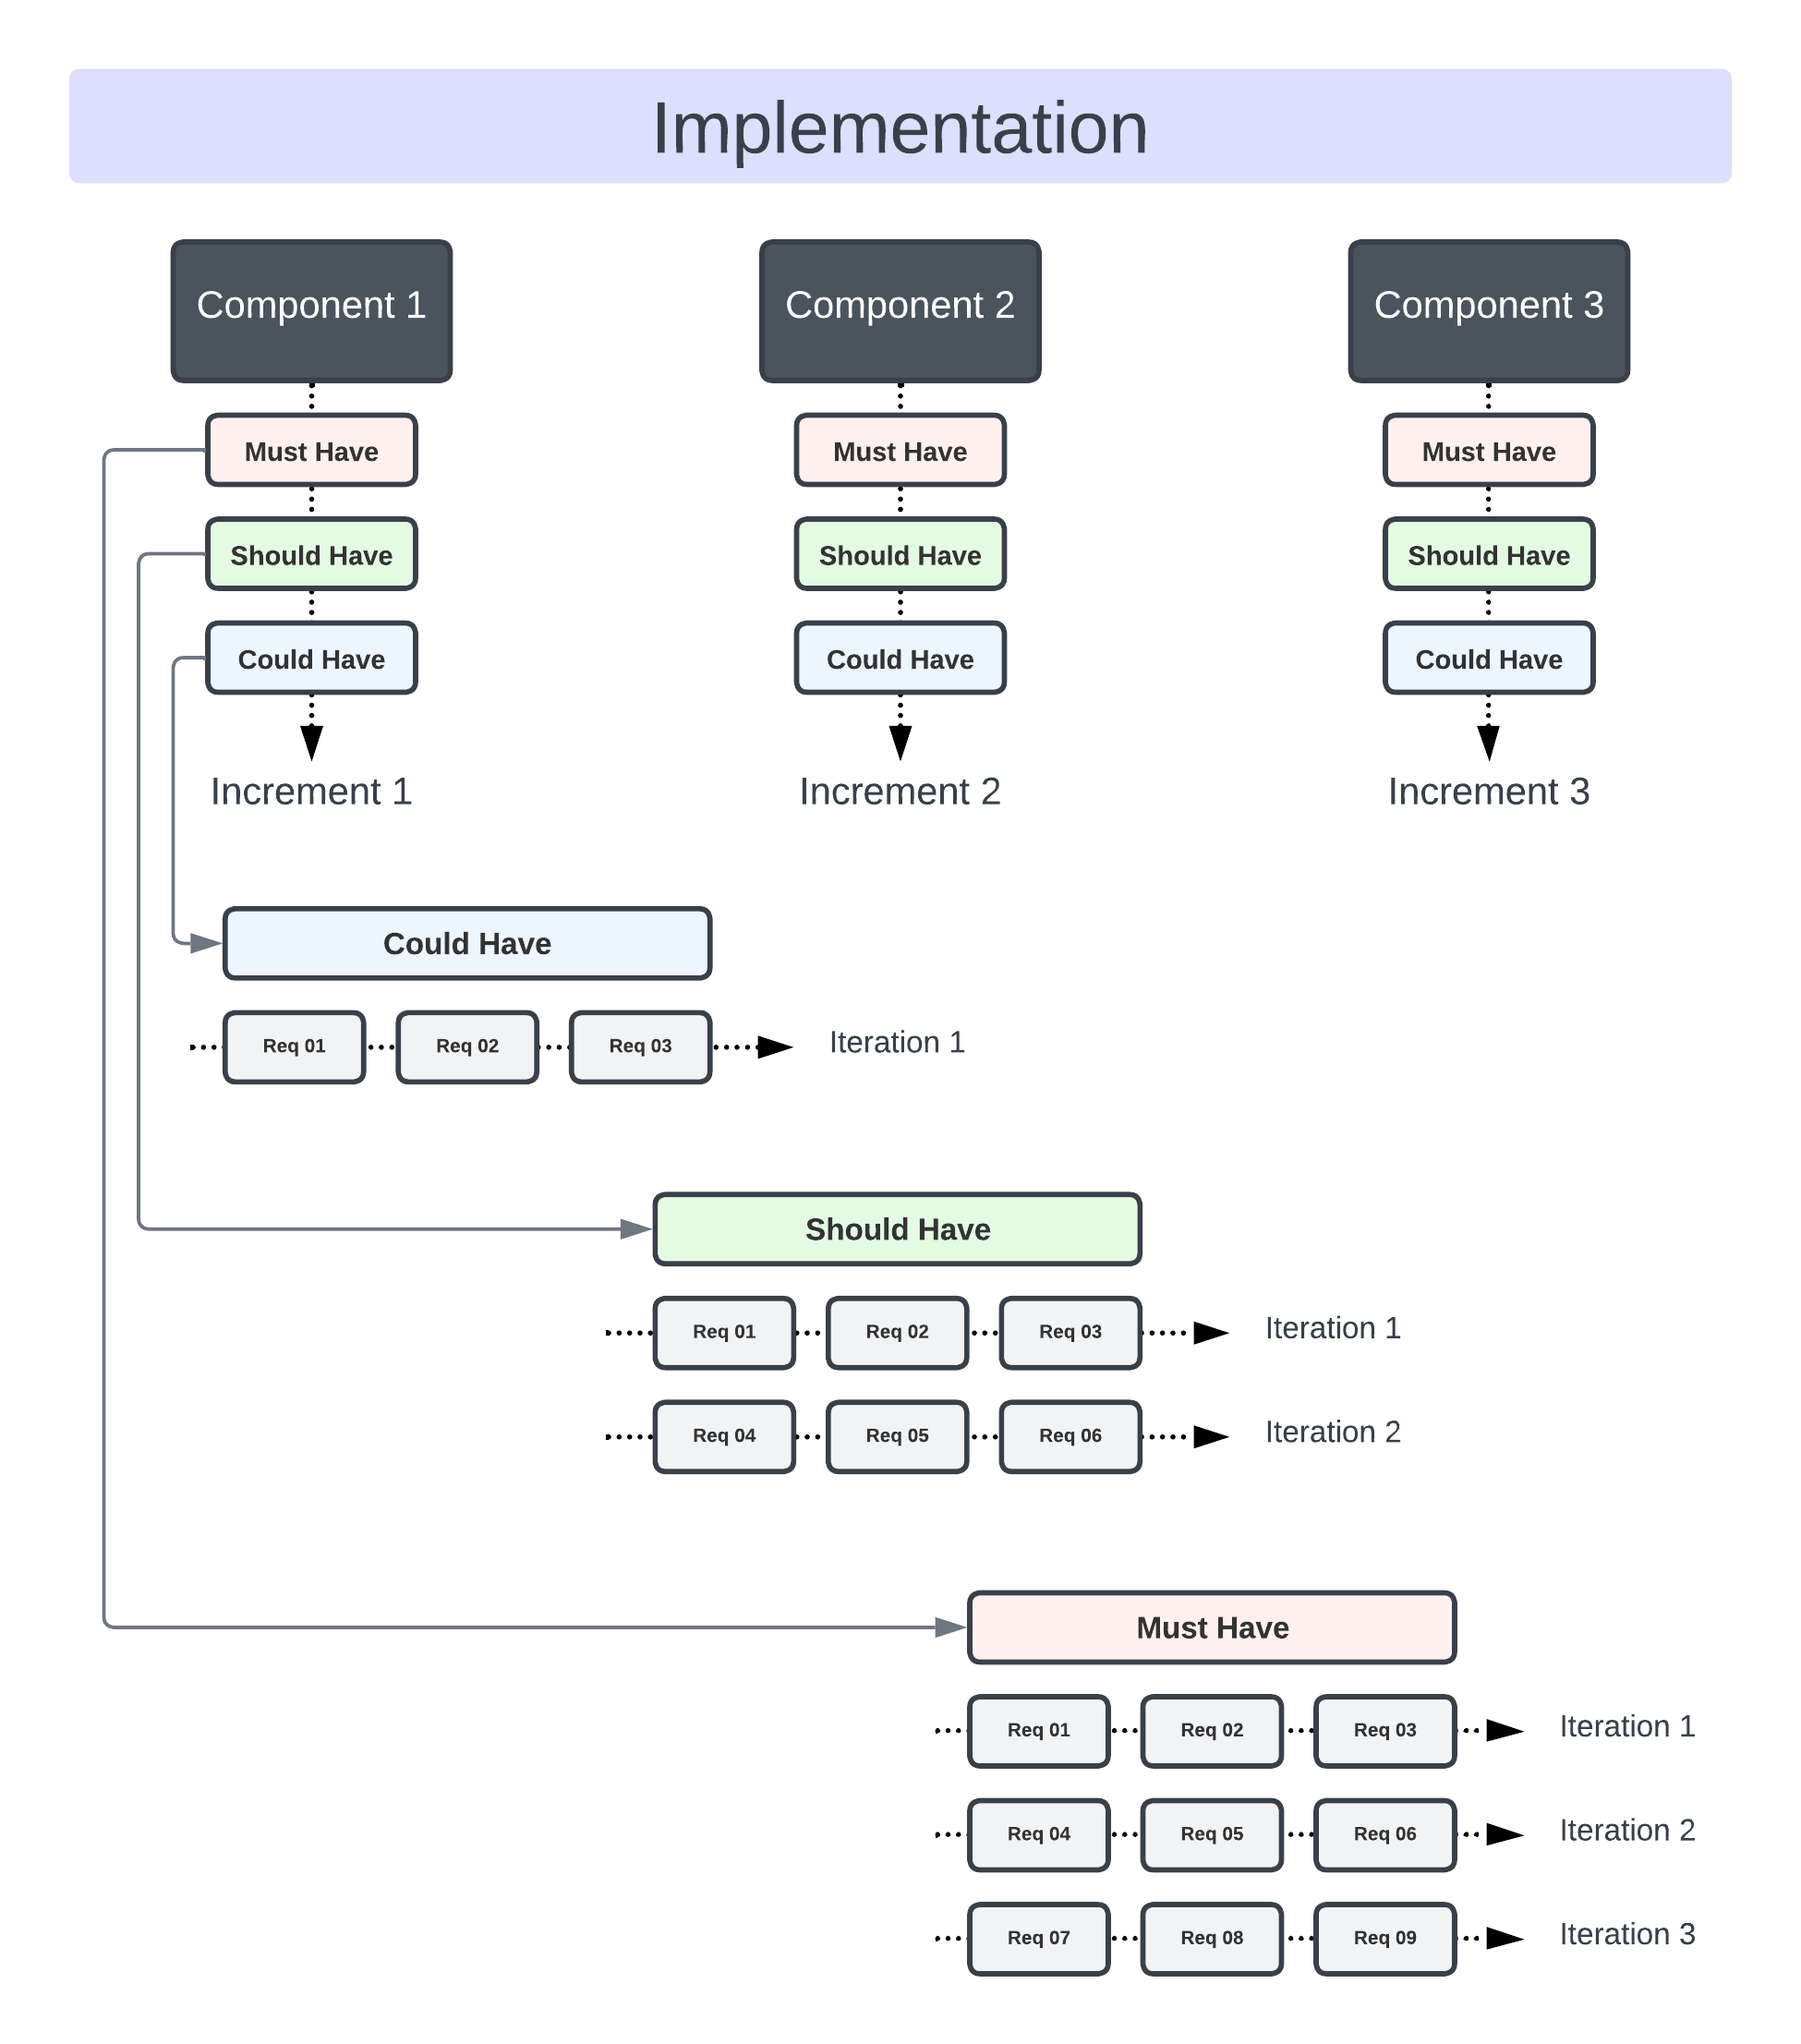
\includegraphics[width=150mm,scale=1]{figures/methodology/ImplementationsApproach.png}}
    \caption{Implementation approach}
    \label{ImplementationsApproach}
\end{figure}

\noindent
Following the phase of implementation, I conduct the testing phase again, which is a continuation of the testing phase that I started in the analysis up to this point. During the testing process at this stage, I determine whether or not the application is able to fulfill the criteria and is suitable for the function for which it was designed. Testing is a crucial part of the quality assurance process since it verifies whether or not the program is dependable, effective, and simple to use. Therefore, I conduct a range of tests to examine the application in its entirety. These tests include both functional and non-functional testing, as well as performance testing.

\vspace{0.25cm}
\newendline Overall, the customized waterfall development strategy that I use enables me to provide an application of high quality that satisfies the needs and requirements that have been set by the stakeholders. I am able to offer a version of the application that is functional at each stage of the incremental and iterative development process, at which point we may collect feedback and make improvements as necessary. Testing activities ensure that the application is reliable, efficient, and user-friendly. They also identify any issues or improvements that need to be made before the application is handed over.\\

\end{justify}

%%%%%%%%%%%%%%%%%%%%%%%%%%%%%%%%%%%%%%%%%%%%%%%%%%%%%%%%%%%%%%%%%%%%%%%%%%%%%%%%%%%%%%%%%%%%%%%%%%%%%%%%%%
\section{Software and Hardware Requirements}
\begin{justify}
It is planned to make use of a wide array of tools, both software, and hardware, in the process of developing this project. Ruby, Ruby on Rails, PostgreSQL, RSpec, React JS, JavaScript, HTML, CSS, Material UI, and Redux are some of the software tools that are available. The application will not only be created using these tools but also tested to guarantee that it is both functional and user-friendly.
\vspace{0.25cm}
\newendline In terms of hardware, a laptop or PC, keyboard, mouse, and internet connection will be required. The laptop or PC will be used as the primary development machine, while the keyboard and mouse will be used for input. An internet connection will be necessary to access online resources and connect to remote development tools.
\vspace{0.25cm}
\newendline In addition, modeling and documentation applications like Lucid chart, Figma, and LaTeX will be used throughout the course of the project. These tools will be used in the production of high-quality documentation for the project, as well as the creation of diagrams and visual models that will be of assistance throughout the analysis and design phase. Last but not least, in order to facilitate the development of the project, a wide range of development tools, such as Visual Studio Code, Git, GitHub, Heroku, and Open-API, will be used. These tools will be used for code management, version control, and deployment, as well as making sure that the program can be seamlessly integrated with other systems.
\end{justify}



\clearpage